\section{Results}
\label{sec:results}

We begin with a demonstrative visual inspection of the \pzpdf s produced by each code for individual galaxies.
Figure~\ref{fig:pz_examples} shows the \pzpdf s for four galaxies chosen as examples of \pzpdf\ archetypes: a narrow unimodal PDF, a broad unimodal PDF, a bimodal PDF, and a multimodal PDF.
We reiterate that under our idealized experimental conditions, differences between the resulting \pzpdf s are the isolated signature of the implicit prior due to the method by which the \pzpdf s were derived.

\begin{figure*}
%\centering
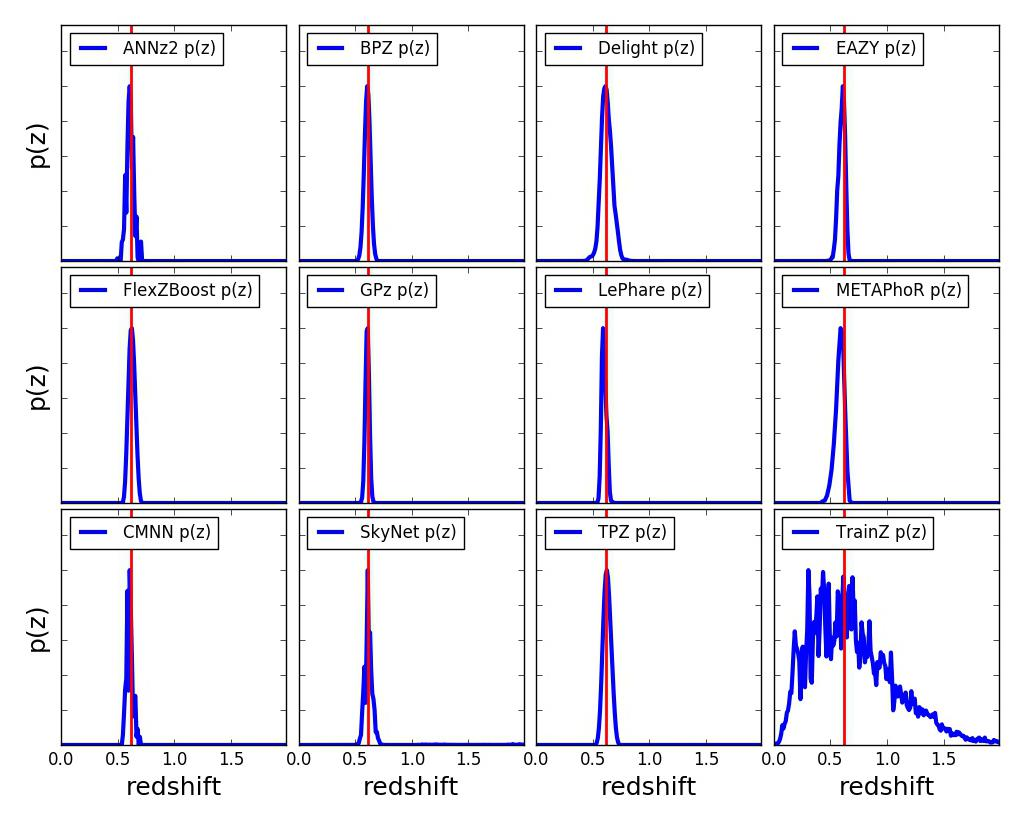
\includegraphics[width=0.49\textwidth]{fig/pz_12codes_261931_noseaborn_crop.jpg}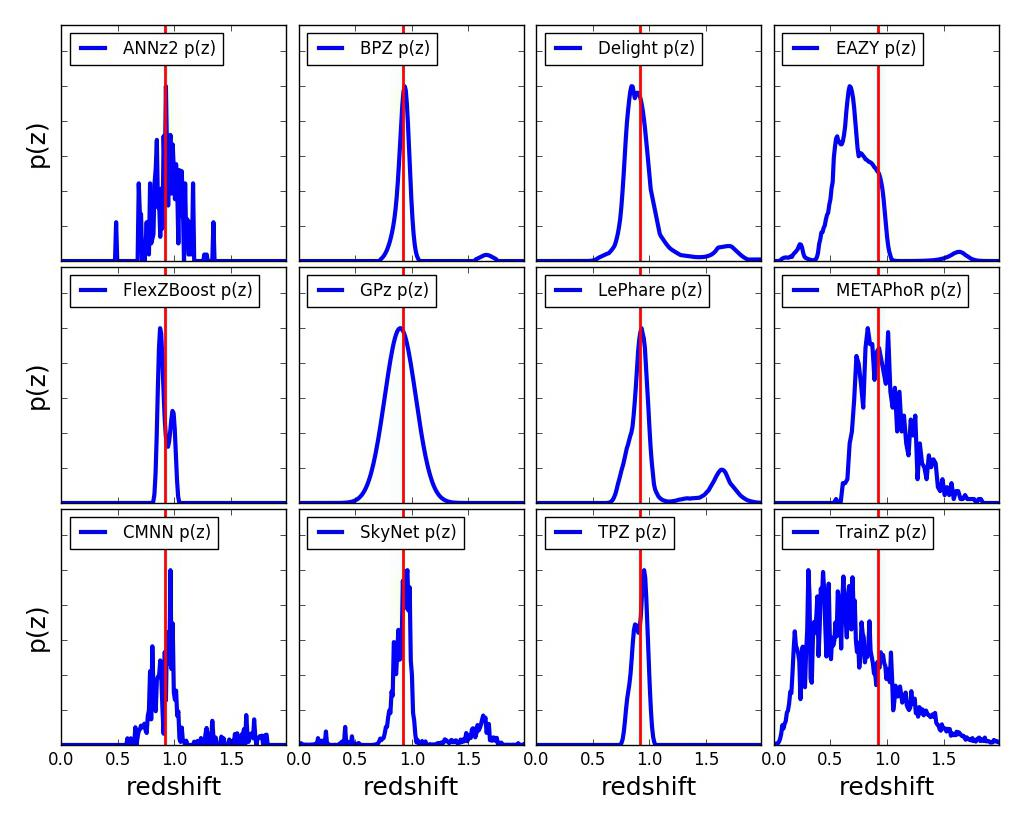
\includegraphics[width=0.49\textwidth]{fig/pz_12codes_471167_noseaborn_crop.jpg}\\
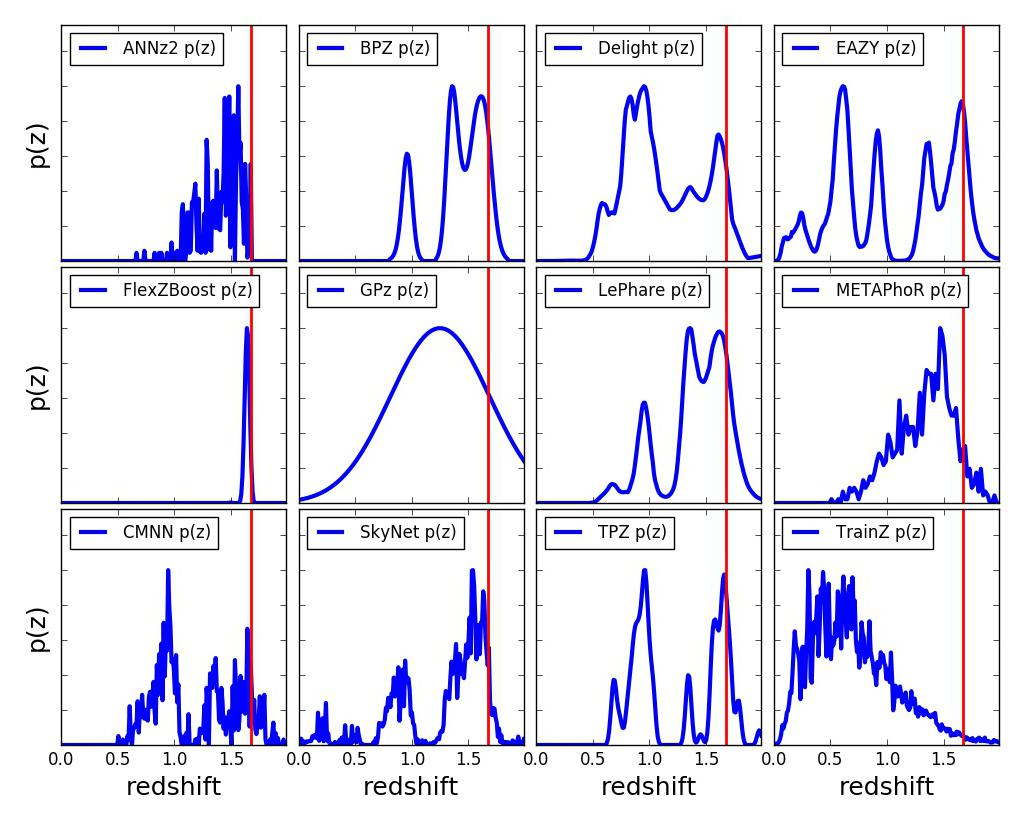
\includegraphics[width=0.49\textwidth]{fig/pz_12codes_713178_noseaborn_crop.jpg}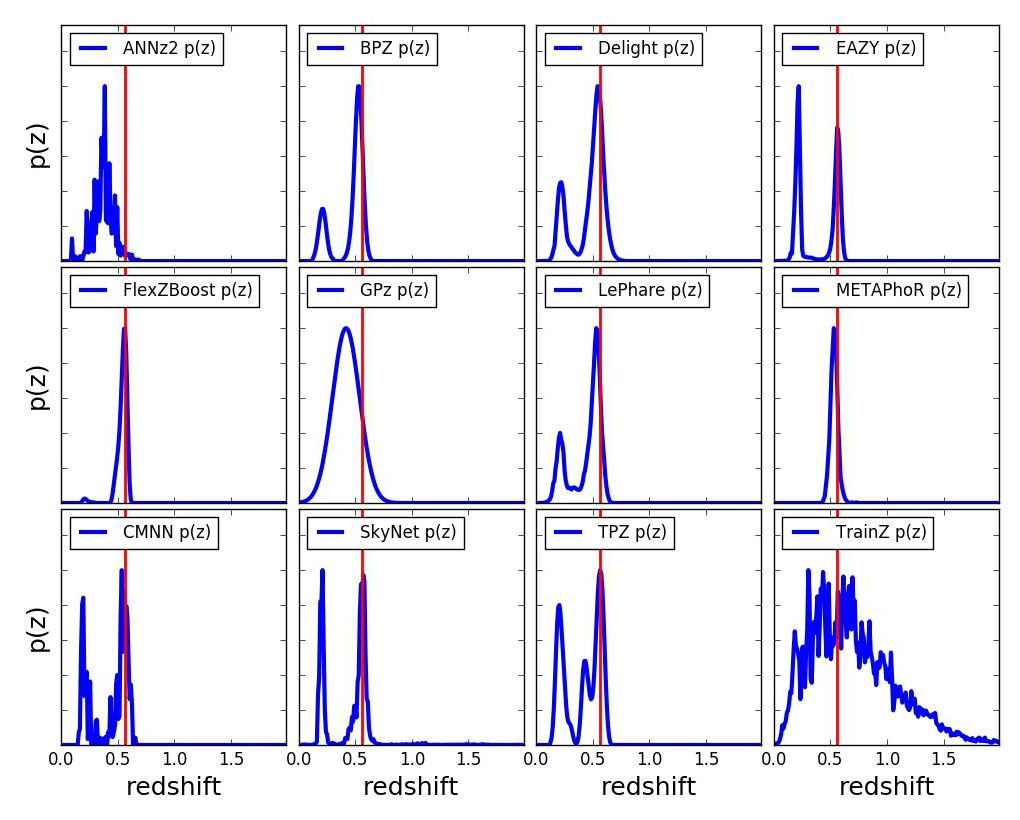
\includegraphics[width=0.49\textwidth]{fig/pz_12codes_982747_noseaborn_crop.jpg}
\caption{The individual \pzpdf s (blue) distributions produced by the twelve codes (small panels) on four exemplary galaxies' photometry (large panels) with different true redshifts (red).
All \pzpdf s have been scaled to the same peak value.
The \pzpdf s of all codes share some features for the example galaxies due to physical colour degeneracies and photometric errors: tight unimodal $p(z)$ (upper left), broad unimodal $p(z)$ (upper right), bimodal $p(z)$ (lower right), and complex/multimodal $p(z)$ (lower left).
The diverse algorithms and implementations induce differences in small-scale structure and sensitivity to physical systematics.}
\label{fig:pz_examples}
\end{figure*}

The most striking differences between codes are the small-scale features induced by the interaction between the shared piecewise constant parameterization of $200$ bins for $0 < z < 2$ of Section~\ref{sec:metrics} and the smoothing conditions or lack thereof in each algorithm.
The $\mathrm{d}z = 0.01$ redshift resolution is sufficient to capture the broad peaks of faint galaxies' \pzpdf s with large photometric errors but is too broad to resolve the narrow peaks for bright galaxies' \pzpdf s with small photometric errors.
This observation is consistent with the findings of \citet[]{Malz:2018} that the piecewise constant form underperforms other parameterizations in the presence of small-scale structures.

However, the shared small-scale features of \annz, \metaphor, \cmnn, and \skynet\ are a result of various weighted sums of the limited number of training set galaxies with colours similar to those of the test set galaxy in question, with behavior closer to classification than regression in the case of \annz.
The settings used on \gpz\ in this work forced broadening of the single Gaussian to cover the multimodal redshift solutions of the other codes.

\subsection{Performance on \pzpdf\ ensembles}
\label{sec:pitqq}

The histogram of PIT values, QQ plot, and QQ difference plot relative to the ideal diagonal are provided in Figure~\ref{fig:pitqq}, showcasing the biases and trends in the average accuracy of the \pzpdf s for each code.
The high QQ values (i.~e.~ more high than low PIT values) of \bpz, \cmnn, \delight, \eazy, and \gpz\ indicate \pzpdf s biased low, and the low QQ values (more low than high PIT values) of \skynet\ and \tpz\ indicate \pzpdf s biased high.
The gray shaded band marks the $2\sigma$ variance in PIT values found using the \trainz\ algorithm with a bootstrap resampling of the training set and a sample size of 30,000 galaxies, representing a very conservative estimate of the representative training sample size estimated as being required for direct \pz\ calibration \citep{Newman:2015}, and thus an approximate minimal error significance compared to ideal performance.
The existence of deviations in the PIT histograms outside of this gray shaded uncertainty range show that significant biases are present for some codes.

\begin{figure*}
\centering
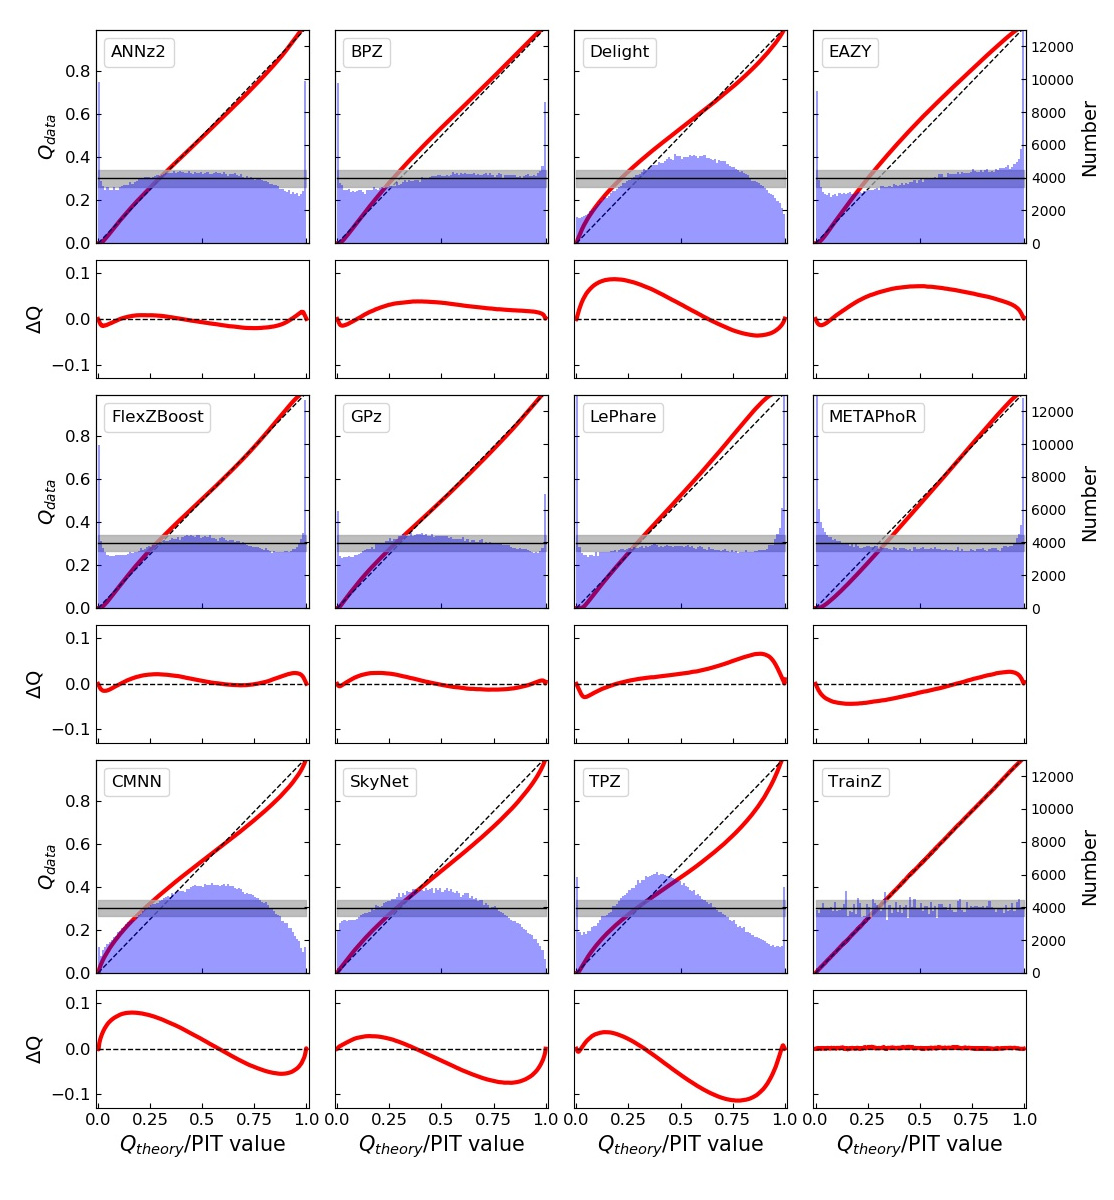
\includegraphics[width=0.74\textwidth]{fig/PITANDQQplot_12codes_withsigmaband_crop.jpg}
\caption{The QQ plot (red) and PIT histogram (blue) of the \pzpdf\ codes (panels) along with the ideal QQ (black dashed diagonal) and ideal PIT (gray horizontal) curves, as well as a difference plot for the QQ difference from the ideal diagonal (lower inset).
The gray shaded region indicates the $2 \sigma$ range from a bootstrap resampling of the training set with a size of 30,000 galaxies using \trainz.
The twelve codes exhibit varying degrees of four deviations from perfection: an overabundance of PIT values at the centre of the distribution indicate a catalogue of overly broad \pzpdf s, an excess of PIT values at the extrema indicates a catalogue of overly narrow \pzpdf s, catastrophic outliers manifest as overabundances at PIT values of 0 and 1, and asymmetry indicates systematic bias, a form of model misspecification.
Values in excess of the $2\sigma$ shaded region show that for some codes these errors will be significant given expected training sample sizes.}
\label{fig:pitqq}
\end{figure*}

The PIT histograms of \delight, \cmnn, \skynet, and \tpz\ feature an underrepresentation of extreme values, indicative of overly broad \pzpdf s, while the overrepresentation of extreme values for \metaphor\ indicates overly narrow \pzpdf s.
These five codes in particular have a free parameter for bandwidth, which may be responsible for this vulnerability, in spite of the opportunity for fine-tuning with perfect prior information.
\flexzboost's ``sharpening'' parameter (described in Section~\ref{sec:flexzboost}) played a key role in diagonalizing the QQ plot, indicating a common avenue for improvement in the approaches that share this type of parameter.
On the other hand, the three purely template-based codes, \bpz, \eazy, and \lephare, do not exhibit much systematic broadening or narrowing, which may indicate that complete template coverage effectively defends from these effects.

\begin{table}
\setlength{\tabcolsep}{2pt}
\centering
\caption{The catastrophic outlier rate as defined by extreme PIT values.
We expect a value of 0.0002 for a proper Uniform distribution.
An excess over this small value indicates true redshifts that fall outside the non-zero support of the $p(z)$.}
\label{tab:pitoutlier}
\begin{tabular}{lc}
\hline
\hline
\Pz\ Code & fraction PIT$<10^{-4}$ or $>$0.9999\\
\hline
\annz       & 0.0265\\
\bpz        & 0.0192\\
\delight    & 0.0006\\
\eazy       & 0.0154\\
\flexzboost & 0.0202\\
\gpz        & 0.0058\\
\lephare    & 0.0486\\
\metaphor   & 0.0229\\
\cmnn       & 0.0034\\
\skynet     & 0.0001\\
\tpz        & 0.0130\\
\hline
\trainz     & 0.0002\\
\end{tabular}
\end{table}

Close inspection of the extremes at PIT values of 0 and 1 reveal spikes in the first and last bin of the PIT histogram for some codes in Figure~\ref{fig:pitqq}, corresponding to catastrophic outliers where the true redshift lies outside of the support of the $p(z)$.
The catastrophic outlier rates are provided in Table~\ref{tab:pitoutlier}.
As expected, \trainz\ achieves precisely the 0.0002 value expected of an ideal PIT distribution.
\annz, \flexzboost, \lephare, and \metaphor\ have notably high catastrophic outlier rates $> 0.02$, exceeding 100 times the ideal PIT rate, meriting further investigation elsewhere.

\begin{figure*}
\centering
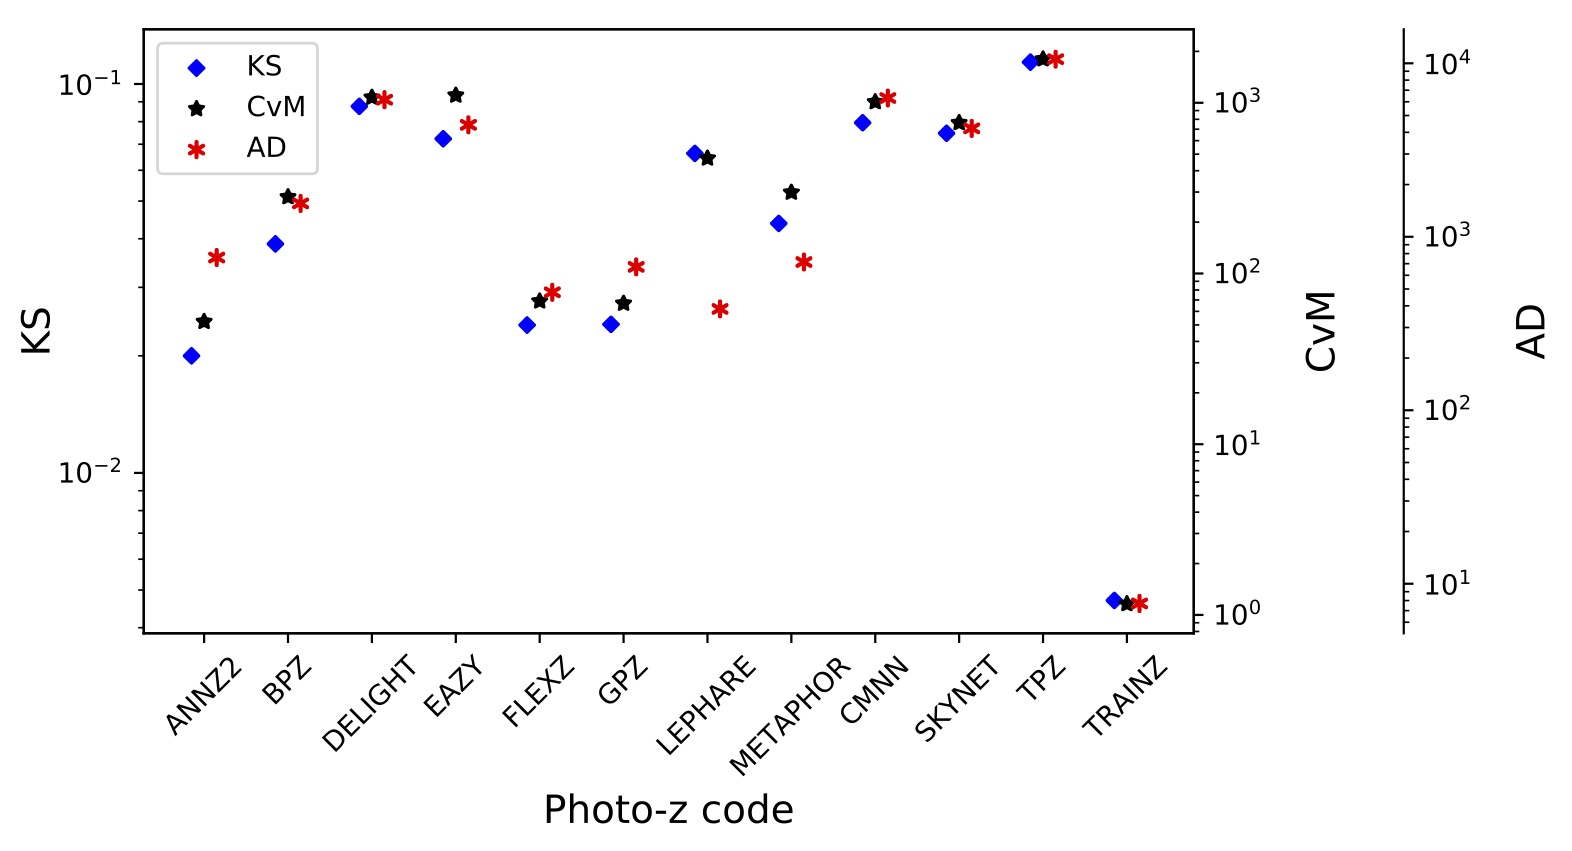
\includegraphics[width=0.74\textwidth]{fig/KSvsCvMvsAD_PIT_withnull_jpg.jpg}
\caption{A visualization of the Kolmogorov-Smirnoff (KS, blue diamond), Cramer-von Mises (CvM, black star), and Anderson-Darling (AD, red asterisk) statistics for the PIT distributions.
There is generally good agreement between these statistics, with differences corresponding to the codes with outstanding catastrophic outlier rates, a reflection of the differences in how each statistic weights the tails of the distribution.
Horizontal lines indicate the level of uncertainty found by bootstrapping a training set sample of 30,000 galaxies using \trainz; none of the codes reach this conservative ideal floor in expected uncertainty.}
\label{fig:pit_stats}
\end{figure*}

Figure~\ref{fig:pit_stats} highlights the relative values of the KS, CvM, and AD test statistics calculated by comparing the PIT distribution and a uniform distribution $U(0, 1)$.
\metaphor\ and \lephare\ perform well under the AD but poorly under the KS and CvM due to their high catastrophic outlier rates.
\annz\ and \flexzboost\  are the top scorers under these metrics of the PIT distribution.
\annz's strong performance can be attributed to an aspect of the training process in which training set galaxies with PIT values that more closely match the percentiles of the DC1 training set's redshift distribution are upweighted; in effect, these quantile-based metrics were part of the algorithm itself that may or may not serve it well under more realistic experimental conditions.
Similar to what was done for the PIT histograms in Figure~\ref{fig:pitqq}, we create bootstrap training samples of 30,000 galaxies for use with \trainz\ in order to estimate a conservative statistical floor that we would expect in real data.
No code reaches this idealized floor, indicating that all codes suffer some degradation from the ideal when employing their implicit priors, though \annz, \flexzboost, and \gpz\ are within a factor of two.

\subsection{Performance on individual \pzpdf s}
\label{sec:cdelossresults}

The values of the CDE loss statistic of individual \pzpdf\ accuracy are provided in Table~\ref{tab:cdeloss}.
It is worth noting that strong performance on the CDE loss, corresponding to lower values of the metric, should imply strong performance on the other metrics, though the inverse is not necessarily true.
Thus the CDE loss is the most effective metric for generic science cases.

\begin{table}  %%% DATA TABLE %%%
\centering
\caption{CDE loss statistic of the individual \pzpdf s for each code.
A lower value of the CDE loss indicates more accurate individual \pzpdf s, with \cmnn\ and \flexzboost\ performing best under this metric.}
\label{tab:cdeloss}
\begin{tabular}{lr}
\hline
Photo-$z$ Code & CDE Loss \\
\hline
\annz 	    & $-6.88$ \\
\bpz 		    & $-7.82$ \\
\delight    & $-8.33$\\
\eazy       & $-7.07$ \\
\flexzboost & $-10.60$\\
\gpz		    & $-9.93$ \\
\lephare 	  & $-1.66$ \\
\metaphor 	& $-6.28$ \\
\cmnn       & $-10.43$ \\
\skynet 	  & $-7.89$ \\
\tpz 		    & $-9.55$ \\
\hline
\trainz		  & $-0.83$ \\
\end{tabular}
\end{table}

Of the metrics we were able to consider in this experiment, \textbf{the CDE Loss is the only metric that can appropriately penalize the pathological \trainz}.
Additionally, it favors \cmnn\ and \flexzboost, the latter of which is optimized for this metric.
